\section{Language Model}\label{sec:model}
In developing this DSL, we needed to have a clear understanding of the specific domain, and develop and appropriate domain model to guide our efforts.  Admittedly, there exist many possible models that can describe this area of policy and policy management, and the model that we chose to initially use is purposefully simple to help ease development and implementation efforts.  We did however provide arbitrary language-level extensibility to support future extension into more demanding policy implementation areas.

We developed this model to help us understand how policy-centric DSLs would be used, to visualize how the various elements are inter-related, and to clarify important areas upon which to focus effort.  Through this model, we were able to conceptualize the initial language structure and generate performance hierarchies, as well as to tailor expected DSL use.

\subsection{Expected Use}
In order to develop the appropriate DSL giving users the power and expressivity they need to easily express usage management concepts, we begin by developing a model describing how we expect it to be used, and by whom, identifying key functional and non-functional characteristics.  We use roles codified as actors to identify the primary user base, and link those roles to specific use cases we expect to be common in day to day DSL use.  We also identify common inputs and outputs from expected activities, and show how those input and output elements are related.  We finally specify the essential core structure of the DSL, as well as extension points and default implementations of those points.

In general day to day use, we expect that certain activities will be much more common that others.  For example, each \textit{policy} requires a \textit{context} in order to both be developed and to run.  That \textit{context} describes the actors using an artifact protected by a policy, the artifact itself, and the environment in which the artifact is both expected to be used (during policy design) and is being used (at evaluation).  That said, the expectation is that the number of policies is much greater than the number of contexts associated with those policies.

Likewise, we expect that the number of times a policy is evaluated is much greater than the number of times that policy is designed and created.  Policies should be read, evaluated, or combined with other policies frequently.  This gives us a magnitude ordering for these activities, where the number of supported contexts is much less than the number of created policies, which is in turn much less than the number of times that policy is evaluated or otherwise used.

This has specific implications on both the DSL syntax and performance profile.  For example, as it is much more common for policies to be evaluated than contexts to be created, our efforts and tuning the system and increasing performance are best focused on policy evaluation rather than contextual activities.  In a similar vein, the language itself should be as simple to comprehend as possible for policies at the expense of contextual elements if necessary.

\begin{figure}[!t]
\centering
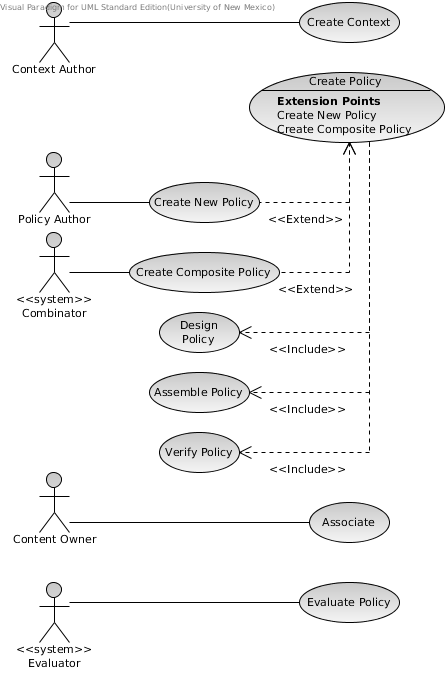
\includegraphics[width=3in]{use-cases}
\caption{General DSL Use Cases}
\label{fig:model:use-cases}
\end{figure}

Figure \ref{fig:model:use-cases} shows the primary system actors we have identified as well as the use cases with which they will be involved.  Actors include:
\begin{itemize}
\item \textit{Context Author}.
\item \textit{Policy Author}.
\item \textit{Combinator}.
\item \textit{Content Owner}.
\item \textit{Evaluator}.
\end{itemize}

\subsection{Domain Ontology}

\begin{figure}[!t]
\centering
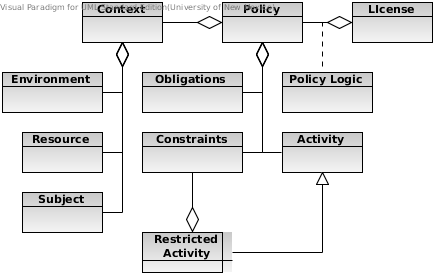
\includegraphics[width=3in]{ontology}
\caption{Basic Language Ontology}
\label{fig:model:ontology}
\end{figure}

\subsection{Envisioned Lifecycle}

\begin{figure}[!t]
\centering
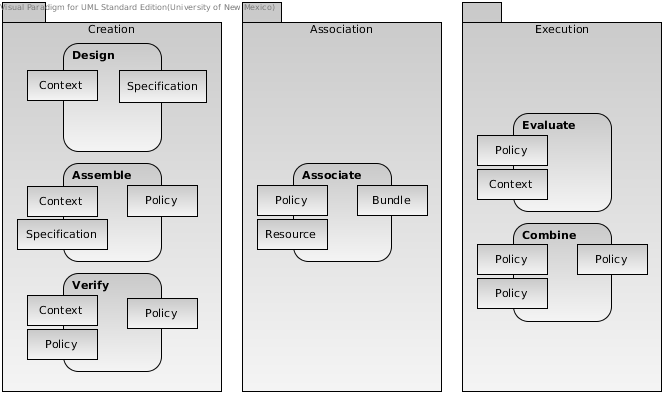
\includegraphics[width=3in]{lifecycle}
\caption{Policy Development Lifecycle}
\label{fig:model:lifecycle}
\end{figure}

\subsection{Language Components}

\begin{figure}[!t]
\centering
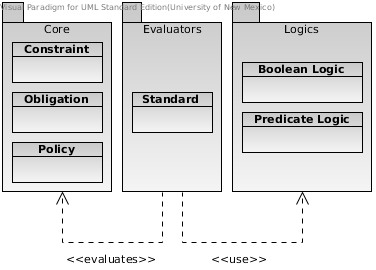
\includegraphics[width=3in]{language-components}
\caption{Language Elements}
\label{fig:model:language-components}
\end{figure}
